\section{Dinámicas factorizables}

En la sección \ref{sec:Ch1PartialTrace} se habló de estados separables como aquellos estados que, descritos por un operador de densidad $\rho\in\densityspace{n}$, tienen la forma
\begin{equation*}
    \rho=\rho_{A}\otimes\rho_{B},
\end{equation*}
donde $\rho_{A}\in\densityspace{m}$, $\rho_{B}\in\densityspace{l}$ y $l+m=n$. Siguiendo esta línea de pensamiento, con \textit{dinámicas factorizables} nos referimos a dinámicas unitarias generadas por hamiltonianos que no contienen un término de interacción (esto es , hamiltonianos de la forma $\mcH=H_{1}\otimes\Id+\Id\otimes H_{2}$), y que por lo mismo son descritas por operadores $\mcU\in\unitaryspace{n}$ que pueden reescribirse como
\begin{equation*}
    \mcU=U_{A}\otimes U_{B}.
\end{equation*}
Aquí, una vez más, $U_{A}\in\unitaryspace{m}$, $U_{B}\in\unitaryspace{l}$ y $l+m=n$. Los operadores separables están compuestos por operadores que actúan de forma independiente sobre diferentes subsistemas del sistema en custión. En el caso de un sistema compuesto por dos subsistemas de dos niveles, el operador separable está compuesto por dos unitarias que actúan sobre $\hilbert_{2}$. Como el estado de máxima entropía resulta ser separable, las dinámicas separables son una muy buena primera forma de aplicar el formalismo descrito en las secciones anteriores.

\subsection{Caso general}

Consideramos una unitaria $\mcU=U_{1}\otimes U_{2}$ que evoluciona en el tiempo como $\mcU_{t}=(U_{1}\otimes U_{2})^{t}=U_{1}^{t}\otimes U_{2}^{t}$. Retomando la ecuación (\ref{eq:MaxEntSeparable}), la evolución del estado de máxima entropía es simplemente
\begin{equation*}
    \varrho_{\max}(t)=U_{1}^{t}\rho_{A}(U_{1}^{t})^{\dag}\otimes U_{2}^{t}\rho_{B} (U_{2}^{t})^{\dag}.
\end{equation*}
De esto, el estado efectivo evolucionado obtenido del principio de máxima entropía, en términos de los multiplicadores de Lagrange es
\begin{equation}\label{eq:SeparableEvolution}
    \rho(t)=pU_{1}^{t}\rho_{A}(U_{1}^{t})^{\dag}+(1-p)U_{2}^{t}\rho_{B} (U_{2}^{t})^{\dag}.
\end{equation}

Por supuesto, esta expresión puede expandirse en términos de exponenciales o de funciones hiperbólicas del vector de Bloch del estado efecivo incial, $\vec{r}_{\rho}$. Si se hace esto para hallar la evolución de un observable $\pauli{i}\in\obspace{2}$ se encuentra que
\begin{align}\label{eq:SeparableEvolutionExpVal}
    \begin{split}
        \expval{\pauli{i}(t)}=&\frac{p\tanh(p\lambda)}{2}\Tr[\pauli{i}U_{1}^{t}(\paulivec{r_{\rho}})(U_{1}^{t})^{\dag}]\\
    &+\frac{p\tanh((1-p)\lambda)}{2}\Tr[\pauli{i}U_{2}^{t}(\paulivec{r_{\rho}})(U_{2}^{t})^{\dag}].
    \end{split}
  \end{align}
En la evolución de los observables (que, depués de todo, son las cantidades que permiten describir al sistema efectivo), se observan, de nueva cuenta, dos términos: el primero está asociado a la evolución de grano grueso sin error. Como el modelo toma en cuenta únicamente a la primera partícula, se espera observar únicamente la acción de la primera parte del operador de evolución separable. El primer término contiene un coeficiente de peso $p\tanh(p\lambda)$ inducido por la aplicación de grano grueso, y el elemento de valor esperado, que depende únicamente de la dirección del vector de Bloch del estado efectivo inicial y de la primera parte del operador de evolución. En contraste, el segundo término contiene la evolución generada por $U_{2}^{t}$, y depende de $(1-p)$, la probabilidad de error. Por esto, este es el término de ruido. Por la naturaleza separable y unitaria de la evolución, se verá que el ruido son oscilaciones periódicas, pero esto es más claro desarrollando algunos ejemplos.

\subsection{Ejemplos particulares}

\subsubsection{Dinámica simétrica}

Comenzamos con el caso en el que la dinámica separable simétrica, esto es, de una unitaria $\mcU\in\unitaryspace{4}$ de la forma
\begin{equation*}
    \mcU_{t}=(U \otimes U)^{t},
\end{equation*}
donde $U\in\unitaryspace{2}$. Se realiza el mismo proceso: aplicamos la evolución al estado de máxima entropía compatible con un conjunto de observables tomográficamente completos en $\hilbert_{2}$ y propagamos al estado con la unitaria subytacente, para luego pasarlo por la aplicación de grano grueso y recuperar el estado efectivo evolucionado. Este caso es quizá el más sencillo, pues la simetría de la unitaria permite factorizarla:
\begin{align*}
\CG{(U^{t}\otimes U^{t})\varrho_{max}(U^{t}\otimes U^{t})^{\dag}}&=pU^{t}\rho_{A}(U^{t})^{\dag}+(1-p)U^{t}\rho_{B}(U^{t})^{\dag} \\
&=U^{t}(p\rho_{A}+(1-p)\rho_{B})(U^{t})^{\dag}\\
&=U^{t}\rho(0)(U^{t})^{\dag}.
\end{align*}
La dinámica efectiva tiene la forma:
\begin{equation}
    \rho\mapsto U^{t}\rho(U^{t})^{\dag}.
\end{equation}

\subsubsection{Identidad de un lado}

Si una de las unitarias que componen a la evolución subyacente es el operador de identidad, el efecto visible en la evolución del estado efectivo depende de la posición de dicha identidad. Supongamos que la evolución microscópica es de la forma $\mcU=U^{t}\otimes\Id$, y que, por lo tanto, deja invariante a la segunda partícula. El estado efectivo se ve como:
\begin{equation}
    \rho\mapsto pU^{t}\rho_{A}(U^{t})^{\dag}+(1-p)\rho_{B}.
\end{equation}
En términos del vector de Bloch del estado efectivo inicial, denotando $r_{A}=\tan(p\lambda)$, $r_{B}=\tan((1-p)\lambda)$, y $O$ la rotación generada por $U$:
\begin{equation*}
    r\hat{r}_{\rho}\mapsto pr_{A}O\hat{r}_{\rho}+(1-p)r_{B}\hat{r}_{\rho}.
\end{equation*}
Esta expresión parece no dar demasiada información: es simplemente la combinación lineal de dos vectores de Bloch, uno que ha sido rotado y otro al que no se le ha hecho nada, pero recordando que el vector de Bloch del estado efectivo inicial cumple $r=pr_{A}+(1-p)r_{B}$, esta puede ser manipulada para ver que
\begin{equation*}
    r\hat{r}_{\rho}\mapsto O(r\hat{r}_{\rho}-(1-p)r_{B}\hat{r}_{\rho})+(1-p)r_{B}\hat{r}_{\rho}.
\end{equation*}
El resultado es una rotación alrededor de una línea que no pasa por el origen. Una rotación de esta naturaleza puede descomponerse en una rotación a través de un eje que pasa por el origen $R$ y una traslación $T$ como $T^{-1}\circ R\circ T$. Notar que una transformación así no tendría por qué mantener a los estados dentro de la esfera de Bloch, por lo que esta debe depender del estado mismo. En efecto, la traslación tiene una magnitud $(1-p)r_{B}$ (a notar que la traslación es pequeña, y corresponde al término de ruido) en la dirección opuesta a la del estado (depende del estado tanto en magnitud como en dirección). Así que, aunque esto podría parecer una transformación afín, no lo es, pues depende enteramente del estado. Como tal, la evolución efectiva no es lineal, y no tiene expresión en términos de operadores de Kraus. La figura \ref{fig:FaseChangeSequence} muestra el efecto que una dinámica de este estilo tiene sobre la esfera de Bloch (en particular, el caso $U=e^{it\pi \pauli{3}}$). La contracción a lo largo del eje $z$ es un resultado del alto valor de $(1-p)$ (0.4), y no sería visible si $p\rightarrow 1$.

\begin{figure}[ht!]
    \centering
    \begin{subfigure}{0.32\textwidth}
      \centering
      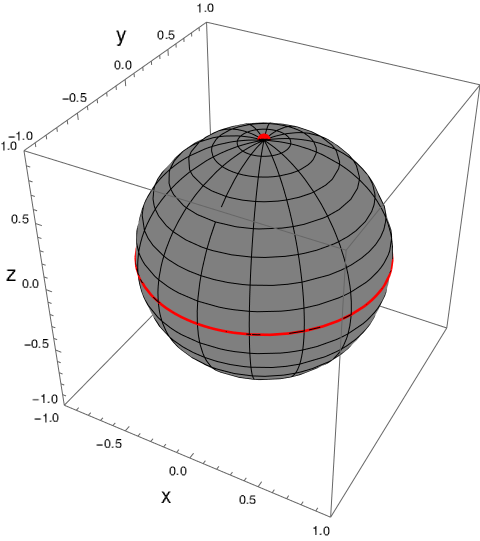
\includegraphics[width=0.9\linewidth]{chapter3/figures_separable/U1xU2_H1=Pi(sz)_H2=Id_z=0.9_p=0.6t=0.png}
      \caption{$t=0.0$}
    \end{subfigure}%
    \begin{subfigure}{0.32\textwidth}
      \centering
      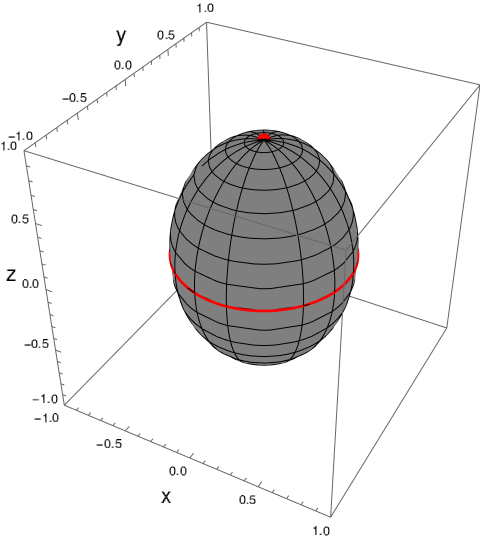
\includegraphics[width=0.9\linewidth]{chapter3/figures_separable/U1xU2_H1=Pi(sz)_H2=Id_z=0.9_p=0.6t=0.25.png}
      \caption{$t=0.25$}
    \end{subfigure}
    \begin{subfigure}{0.32\textwidth}
      \centering
      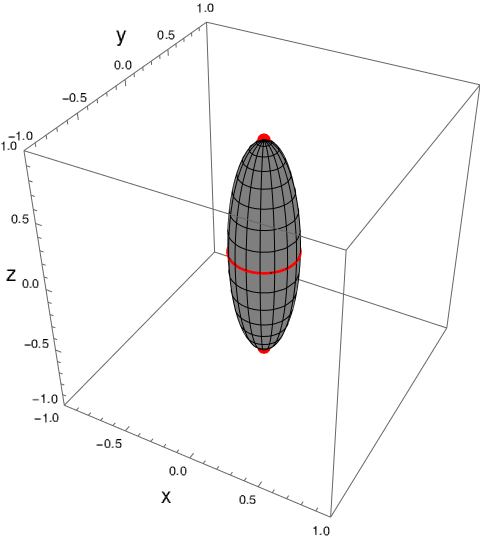
\includegraphics[width=0.9\linewidth]{chapter3/figures_separable/U1xU2_H1=Pi(sz)_H2=Id_z=0.9_p=0.6t=0.5.png}
      \caption{$t=0.5$}
    \end{subfigure}
    \caption{Efecto de la evolución subyacente sobre la esfera de Bloch si $r=0.9$, $p=0.6$ y $U_{1}=e^{it\pi \pauli{3}}$. La dramática contracción a lo largo de $z$ se asocia al alto valor de $1-p$.}
    \label{fig:FaseChangeSequence}
\end{figure}

Si, por otro lado, la dinámica es de la forma $\mcU=\Id\otimes U^{t}$, esta puede ser escrita en términos de los vectores de Bloch como
\begin{equation*}
    r\hat{r}_{\rho}\mapsto pr_{A}O\hat{r}_{\rho}+(1-p)r_{B}\hat{r}_{\rho}.
\end{equation*}
Con algunas manipulaciones, la evolución toma una forma más clara:
\begin{equation*}
    r\hat{r}_{\rho}\mapsto r\hat{r}_{\rho}+(1-p)(O(r_{B}\hat{r}_{\rho})-r_{B}\hat{r}_{\rho}).
\end{equation*}
En este caso, el primer término es el término invariante, y sería lo único visible en el caso en que el aparato de medición no fallara, mientras que el segundo término corresponde a pequeñas oscilaciones completamente dependientes del estado efectivo inicial. Estas pequeñas oscilaciones son el término de ruido, y por su dependencia en el estado inicial, vuelve a suceder que la evolución no es lineal, y que no tiene representación en términos de operadores de Kraus.

\subsubsection{Cambio de fase con oscilaciones}

Considérese un estado efectivo $\rho\in\densityspace{2}$ de la forma
\begin{equation*}
    \rho(0)=\frac{1}{2}(\Id+r\pauli{3}),
\end{equation*}
asociado a un sistema microscópico de estado $\varrho\in\densityspace{4}$, y que la evolución que experimenta dicho sistema es
\begin{equation*}
    \mcU=e^{-itH_{1}}\otimes e^{-itH_{2}},
\end{equation*}
donde
\begin{align*}
    H_{1}=\pauli{1} & & y & &H_{2}=\frac{\omega}{\sqrt{2}}(\pauli{1}-\pauli{2}).
\end{align*}

El estado de máxima entropía asociado al estado efectivo inicial es el dado por la ecuación (\ref{eq:MaxEntSeparable}). En términos de la catidad observable $r$, y con ayuda de la función $f$ dada por (\ref{eq:r(lambda)}), la evolución del estado de máxima entropía es
\begin{equation*}
    \varrho(t)=\frac{1}{2}\qty(\Id+p\tanh(pf^{-1}(r))\pauli{3}e^{itH_{1}})\otimes\frac{1}{2}\qty(\Id+(p-1)\tanh((p-1)f^{-1}(r))e^{-itH_{2}}\pauli{3}e^{itH_{2}}).
\end{equation*}
El estado efectivo obtenido a través de la aplicación de grano grueso escrita
\begin{align*}
    \rho(t)=&\frac{p}{2}\qty(\Id+p\tanh(pf^{-1}(r))e^{-itH_{1}}\pauli{3}e^{itH_{1}})\\
    &+\frac{(1-p)}{2}\qty(\Id+(p-1)\tanh((p-1)f^{-1}(r))e^{-itH_{2}}\pauli{3}e^{itH_{2}}).
\end{align*}
El valor esperado de $\pauli{3}$, puede hallarse gracias a la ecuación (\ref{eq:SeparableEvolutionExpVal}), siendo particularmente útil la ecuación (\ref{ap:PauliCompExp}) para desarrollar a ambas unitarias. En efecto, estas tienen representación matricial
\begin{align*}
    U_{1}^{t}=\begin{pmatrix}
        \cos(t)+i\sin(t) & 0\\
        0 & \cos(t)-i\sin(t)
    \end{pmatrix}& & y & & U_{2}^{t}=\begin{pmatrix}
        \cos(\omega t) &-\frac{1+i}{\sqrt{2}}\sin(\omega t) \\
        \frac{1-i}{\sqrt{2}}\sin(\omega t) & \cos(\omega t)
    \end{pmatrix}.
\end{align*}
En el caso en que no hubiera error, uno esperaría que el valor esperado de $\pauli{3}$ fuera precisamente $r$ para cualquier tiempo, ya que el cambio en la fase relativa en el primer subsistema no es observable, sin embargo, en este caso se halla que
\begin{equation*}
    \expval{\pauli{3}(t)}=r+(1-p)r_{B}(\cos(2\omega t)-1).
\end{equation*}
\begin{figure}[ht!]
    \centering
    \begin{subfigure}{0.5\textwidth}
      \centering
      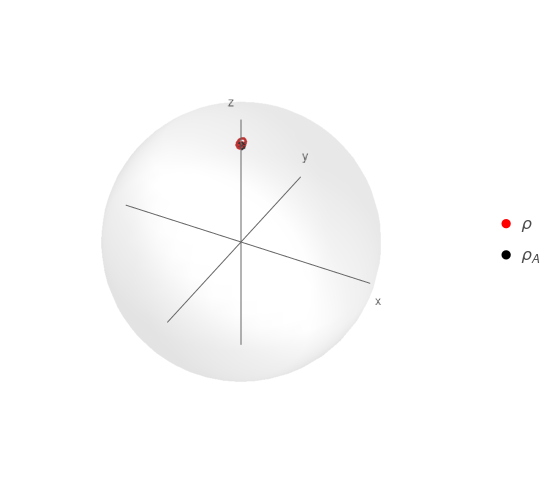
\includegraphics[width=0.9\linewidth]{chapter3/figures_separable/U1xU2_H1=(sz)_H2=15(sx-sy)_z=0.8_p=0.9_far.png}
      \caption{$t=0.0$}
    \end{subfigure}%
    \begin{subfigure}{0.5\textwidth}
      \centering
      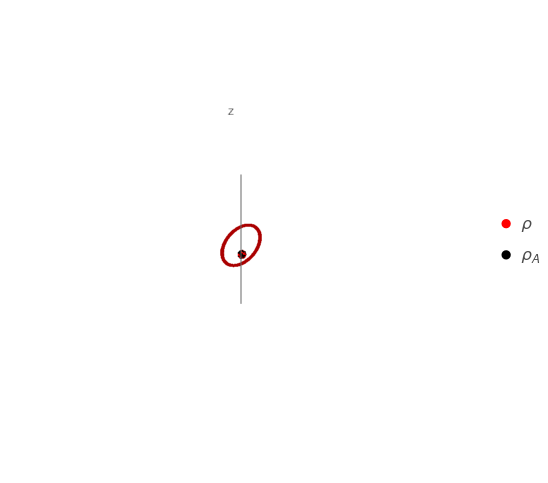
\includegraphics[width=0.9\linewidth]{chapter3/figures_separable/U1xU2_H1=(sz)_H2=15(sx-sy)_z=0.8_p=0.9.png}
      \caption{$t=0.25$}
    \end{subfigure}
    \caption{Oscilaciones cercanas al valor esperado, para cuando $r=r_{z}=0.8$, $p=0.9$ y $\omega=15$. }\label{fig:EvolutionOscilations}
\end{figure}

Este resultado puede observarse en la figura \ref{fig:EvolutionOscilations}, donde se observa que la evolución efectiva se ve como oscilaciones alrededor de un punto cercano al estado del primer subsistema, $\rho_{A}$. Aunque en este caso, el primer subsistema no experimenta cambios, pues es invariante bajo la unitaria $U_{1}$, estas oscilaciones son visibles en casos más generales, como puede observarse en la figura \ref{fig:GeneralOscilations1}.

\begin{figure}[ht!]
    \centering
    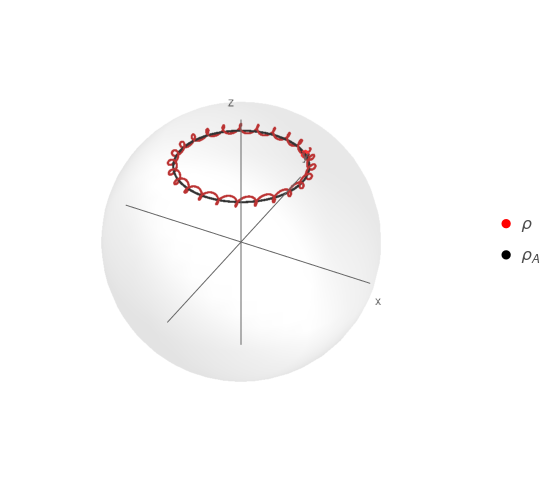
\includegraphics[width=0.6\linewidth]{chapter3/figures_separable/U1xU2_H1=(sz)_H2=15(sx-sy)_z=0.8_p=0.9_wXY=0.5.png}
    \caption{Oscilaciones cercanas al valor esperado. En este caso, el estado inicial no se halla alineado en $z$, por lo que $U_{1}$ lo rota alrededor de dicho eje. Aquí, $r=0.8$ $p=0.9$ y $\omega=15$. }
    \label{fig:GeneralOscilations1}
\end{figure}
